\documentclass[main.tex]{subfiles}


% Cowan_2011
\begin{document}

\section{Overview}

This analysis utilizes a binned liklihood-maximization technique comparing some observation, whether it is true data or pseudodata, against Monte Carlo simulation weighted to the expectation from multiple sterile neutrino hypothesis. 
Binning is done on reconstructed quantities; bins are linearly spaced in $\cos\theta_{reco}$ and logarithmically spaced in $E_{reco}$. 
Sterile neutrino points are chosen uniformly over $\left|U_{\mu 4}\right|^{2}=\sin^{2}\theta_{24}$, $\left|U_{\tau 4}\right|^{2}=\sin^{2}\theta_{34}\cos^{2}\theta_{24}$, and $\Delta m_{41}^{2}$. 
A 16 by 16 grid in the unitary mixing matrix elements, and five discrete mass-squared splittings are explored. 
These five values are 
\begin{enumerate}
    \item 1.0eV$^{2}$ - a commonly chosen value used in sterile oscillations studies. 
    \item 3.5eV$^{2}$ - a value close to the best-fit point from BEST~\cite{barinov2021results}
    \item 4.5eV$^{2}$ - a value close to the eight-year IceCube through-going track analysis~\cite{Aartsen_2020, Aartsen_2020_prd}
    \item 10.0eV$^{2}$ - an intermediate value between those above, and larger mass-squared splitting
    \item 100.0eV$^{2}$ - a larger mass-squared splitting where fast oscillations will dominate the signal. 
\end{enumerate}

\section{Likelihood Metric}

The likelihood used in this analysis is defined as the probability of observing a given set of data, or pseudodata, assuming some physics hypothesis.
It is quantified as 
\begin{equation}
    \mathcal{L}(\vec{\Theta}, \vec{\eta}) = \prod_{i=0}^{\text{bins}} \mathcal{L}_{eff}\left( w_{i}^{sum}, w_{2,i}^{sum}, k_{i} \right),
\end{equation}
where $w_{i}$ and $w_{2,i}$ are the sums of the MC weights and MC weights squared, respectively, in bin $i$; $k_{i}$ is the observed number of events (or pseudoevents). 
$\vec{\Theta}$ is the tested physics hypothesis and $\vec{\eta}$ the set of nuisance parameters. 

The effective likelihood function, defined in Ref~\ref{effective_llh}, is part of a family of likelihood metrics used to account for MC statistical uncertainty. 
We use the form where
\begin{align}
    \alpha&=\dfrac{\mu^{2}}{\sigma^{2}} +1 & &\text{and} & \beta&=\dfrac{\mu}{\sigma^{2}}.
\end{align}
Since each simulated MC event is just one event, $\mu = w_{i}$ and $\sigma^{2} = w_{2,i}$\footnote{it is possible to merge MC events into `meta-events' to speed up reweighting, where the functional forms are slightly more complicated. This, however, is not done in this analysis}, and
\begin{equation}
    \mathcal{L}_{eff}(\vec{\Theta} | k) = \left(\dfrac{\mu}{\sigma^{2}}\right)^{\tfrac{\mu^{2}}{\sigma^{2}} + 1} \Gamma\left(k + \dfrac{\mu^{2}}{\sigma^{2}} + 1\right) \left[ k! \left(1+\dfrac{\mu}{\sigma^{2}}\right)^{k+\tfrac{\mu^{2}}{\sigma^{2}} + 1} \Gamma\left(\dfrac{\mu^{2}}{\sigma^{2}} +1\right)\right]^{-1}
\end{equation}
where $\Gamma$ is the gamma function. 

The set of nuisance parameters describe that describe systematic uncertainties are themselves constrained by Gaussian priors functions. 
These priors are used to weight the likelihoods, which is maximized to form a profile likelihood, defined as 

\begin{equation}
\mathcal{L}_{\text{profile}}\left(\vec{\theta}\right) = \text{max}_{\vec{\eta}}\left[\mathcal{L}(\vec{\Theta}, \vec{\eta}) \Xi(\vec{\eta}) \right]
\end{equation}
where $\Xi(\vec{\eta})$ is the total likelihood penalty for the set of nuisance parameters $\vec{\eta}$ calculated accounting for the correlations between the priors. 

We then construct an analysis test statistic (TS) for producing convidence intervals, which we define as 
\begin{equation}\begin{split}
TS(\vec{\Theta}) &= -2\left[ \log\mathcal{L}_{\text{profile}}(\vec{\theta}) - \log\mathcal{L}_{\text{profile}}(\vec{\Theta}_{min}) \right] \\
&= -2 \Delta \log\mathcal{L}_{\text{profile}}(\vec{\theta})\\
&=-2\Delta \text{LLH}
\end{split}\end{equation}
where $\vec{\Theta}_{min}$ is the sterile hypothesis that maximizes the likelihood, and best matches the data: the best fit point. 

\section{Tests}

A series of tests were performed to validate the implementation of the nuisance parameters and verify the performance of the fitting framework. 

\subsection{Inject-Recover Systematic Tests}

Pseudo-experimental results, or `realizations,' are first calculated by perturbing each nuisance parameter some amount, individually, and getting the expected event rates without additional statistical variation applied. 
This is done for each nuisance parameter allowed to float in the fit, for various amounts chosen in the allowed range given by the parameters' priors. 
Fits are then carried out to each of these realizations.
The results are tabulated below in Figure FIG. 

\subsection{Asimov Sensitivity}



\subsection{Systematic Impact Tests}

Nuisance parameters were collected into ``bundles.'' 
Asimov sensitivity scans~\cite{Cowan_2011} were then performed for each bundle while fixing the parameters of that bundle to their central values.
The resulting confidence intervals then show the impact of fixing those nuisance parameters. 
The bundles are 
\begin{enumerate}
    \item Conv(entional): Daemonflux~\cite{yanez2023daemonflux} parameters, AIRS scale, and the kaon-nucleon cross section uncertainty
    \item Astr: astrophysical normalization and the spectral index
    \item Det(ector): hole ice uncertainty, DOM efficiency, and the bulk-ice uncertainty
    \item Muon: the CR muon background\footnote{Because of the large, extra, error introduced by the muon background, for this systematic impact test a special realization is generated and fit to where there no muon contribution is added at all.}
    \item Normalization (aeff\_scale): overall normalization
\end{enumerate}
These sensitivities are shown, for 90\% CL and 3 degrees of freedom in Figure~\ref{fig:impact}

\begin{figure}
    \centering
    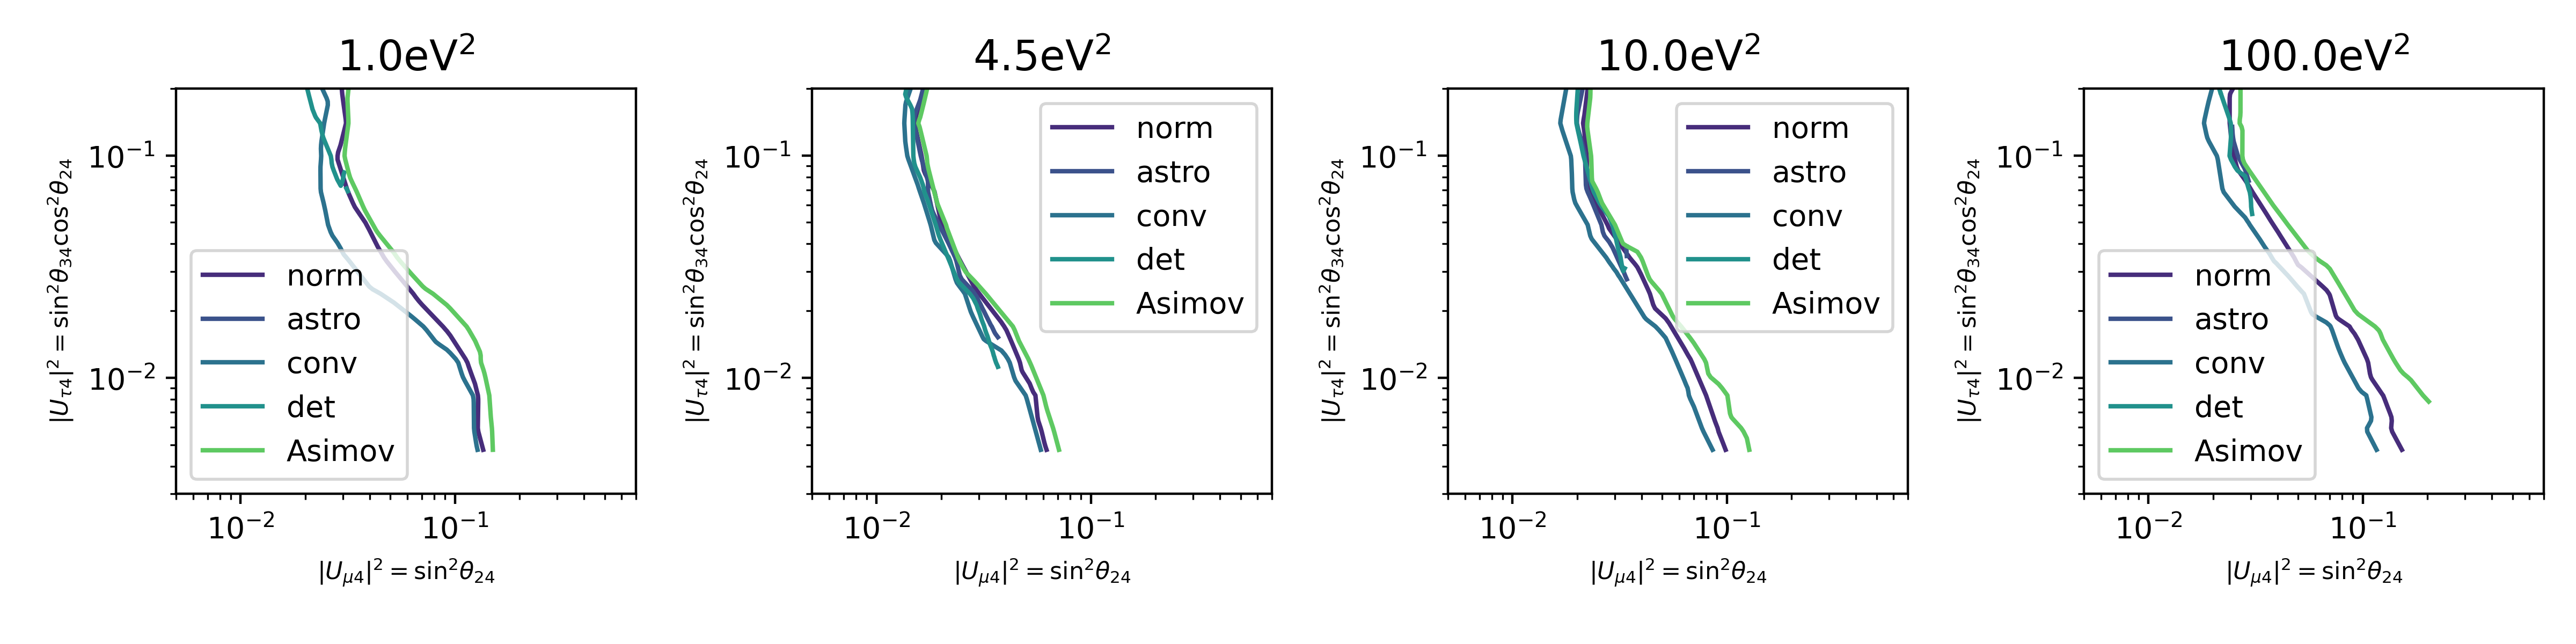
\includegraphics[width=0.90\linewidth]{figures/systematic_impact.png}
    \caption{The sensitivity contours for fixing each bundle of nuisance parameters. Contours are shown at 90\% CL and 3DOF for various mass-squared splittings; from left to right: 1.0eV$^{2}$, 4.5eV$^{2}$, 10.0eV$^{2}$, and 100.0eV$^{2}$.}\label{fig:impact}
\end{figure}


\end{document}